% Options for packages loaded elsewhere
\PassOptionsToPackage{unicode}{hyperref}
\PassOptionsToPackage{hyphens}{url}
\documentclass[
]{article}
\usepackage{xcolor}
\usepackage{amsmath,amssymb}
\setcounter{secnumdepth}{-\maxdimen} % remove section numbering
\usepackage{iftex}
\ifPDFTeX
  \usepackage[T1]{fontenc}
  \usepackage[utf8]{inputenc}
  \usepackage{textcomp} % provide euro and other symbols
\else % if luatex or xetex
  \usepackage{unicode-math} % this also loads fontspec
  \defaultfontfeatures{Scale=MatchLowercase}
  \defaultfontfeatures[\rmfamily]{Ligatures=TeX,Scale=1}
\fi
\usepackage{lmodern}
\ifPDFTeX\else
  % xetex/luatex font selection
\fi
% Use upquote if available, for straight quotes in verbatim environments
\IfFileExists{upquote.sty}{\usepackage{upquote}}{}
\IfFileExists{microtype.sty}{% use microtype if available
  \usepackage[]{microtype}
  \UseMicrotypeSet[protrusion]{basicmath} % disable protrusion for tt fonts
}{}
\makeatletter
\@ifundefined{KOMAClassName}{% if non-KOMA class
  \IfFileExists{parskip.sty}{%
    \usepackage{parskip}
  }{% else
    \setlength{\parindent}{0pt}
    \setlength{\parskip}{6pt plus 2pt minus 1pt}}
}{% if KOMA class
  \KOMAoptions{parskip=half}}
\makeatother
\usepackage{graphicx}
\makeatletter
\newsavebox\pandoc@box
\newcommand*\pandocbounded[1]{% scales image to fit in text height/width
  \sbox\pandoc@box{#1}%
  \Gscale@div\@tempa{\textheight}{\dimexpr\ht\pandoc@box+\dp\pandoc@box\relax}%
  \Gscale@div\@tempb{\linewidth}{\wd\pandoc@box}%
  \ifdim\@tempb\p@<\@tempa\p@\let\@tempa\@tempb\fi% select the smaller of both
  \ifdim\@tempa\p@<\p@\scalebox{\@tempa}{\usebox\pandoc@box}%
  \else\usebox{\pandoc@box}%
  \fi%
}
% Set default figure placement to htbp
\def\fps@figure{htbp}
\makeatother
\setlength{\emergencystretch}{3em} % prevent overfull lines
\providecommand{\tightlist}{%
  \setlength{\itemsep}{0pt}\setlength{\parskip}{0pt}}
\usepackage{bookmark}
\IfFileExists{xurl.sty}{\usepackage{xurl}}{} % add URL line breaks if available
\urlstyle{same}
% fallback for those not using the hyperref driver hyperxmp:
\makeatletter
\@ifundefined{xmpquote}{\newcommand{\xmpquote}[1]{#1}}{}
\makeatother
\hypersetup{
  hidelinks,
  pdfcreator={LaTeX via pandoc}}

\author{}
\date{}

\begin{document}

\section{Lab 2: Linguistics Data}\label{lab-2-linguistics-data}

\subsection{1. Introduction}\label{introduction}

This analysis examines regional variation in language use across the
United States. In particular, I am interested in how linguistic
responses differ across geographic areas and whether people can be
grouped into meaningful clusters based on similarities in their language
use.

Identifying such clusters may reveal groups of regions that share
similar linguistic patterns even when they are not geographically
adjacent. If comparable data were available over time, it would also be
interesting to examine how these linguistic groups change. However, the
current dataset does not provide this temporal dimension.

In this analysis, I first explore the geographic patterns of selected
linguistic responses. I then use dimension reduction and clustering
methods to examine whether respondents with similar patterns of word use
can be divided into distinct groups, how many groups are supported by
the data, and how stable these groupings are.

\subsection{2. The Data}\label{the-data}

The data come from Bert Vaux's Dialect Survey and contain responses from
47,471 respondents across the United States. The individual-level
dataset contains respondent ID, self-reported city and state, ZIP code,
latitude and longitude, and responses to a set of dialect survey
questions.

This analysis focuses on the lexical questions numbered Q50--Q121. The
survey responses are categorical. A value of 0 indicates that the
respondent did not answer the question, while the other numerical values
correspond to different response choices.

Respondents from different geographic areas answered the same set of
questions about their language use. These responses provide information
about differences in word choice and other patterns of language use
across individuals. Because geographic information is available for the
respondents, linguistic similarities can be compared with geographic
patterns. Individuals can therefore be clustered based on similarities
in their linguistic responses, and the resulting clusters can then be
examined to determine whether they correspond to meaningful geographic
patterns.

However, the survey does not necessarily provide a representative sample
of the U.S. population, so geographic patterns should be interpreted as
patterns within the observed survey respondents rather than precise
population estimates.

\subsubsection{2.1 Data Cleaning}\label{data-cleaning}

I first selected and explored the 67 survey questions included in the
dataset. Because the original responses were categorical, I converted
each response category into binary indicator variables using one-hot
encoding. This initially produced 535 binary variables. A response value
of 0 represents a missing or unanswered question rather than an actual
linguistic response. I therefore removed the 67 binary columns
corresponding to response 0, leaving 468 binary linguistic features. I
also examined the number of answered questions for each respondent.
Although most respondents answered all 67 questions, some respondents
had missing responses.

The missing responses were particularly important for dimension
reduction. In the initial PCA using all respondents, the third principal
component was strongly associated with the number of questions answered
(correlation approximately 0.54). This suggested that part of the PCA
structure reflected response completeness rather than linguistic
variation.

For the main PCA and clustering analyses, I therefore restricted the
data to the 40,061 respondents who answered all 67 questions. This
allowed the later analyses to focus more directly on variation in
linguistic responses rather than variation in missingness.

\subsubsection{2.2 Exploratory Data
Analysis}\label{exploratory-data-analysis}

I first examined Q68 and Q69, which ask respondents what terms they use
for their maternal and paternal grandmothers. I selected these two
questions because they measure closely related linguistic choices,
allowing me to examine both the relationship between responses and their
geographic variation.

The responses showed noticeable geographic variation. ``Granny'' was
relatively more common in Southern and Southeastern states, including
Tennessee, Alabama, and Kentucky, whereas ``nana'' was relatively more
common in the Northeast, particularly in New England. Similar geographic
patterns appeared for both maternal and paternal grandmother
terminology.

\begin{figure}
\centering
\pandocbounded{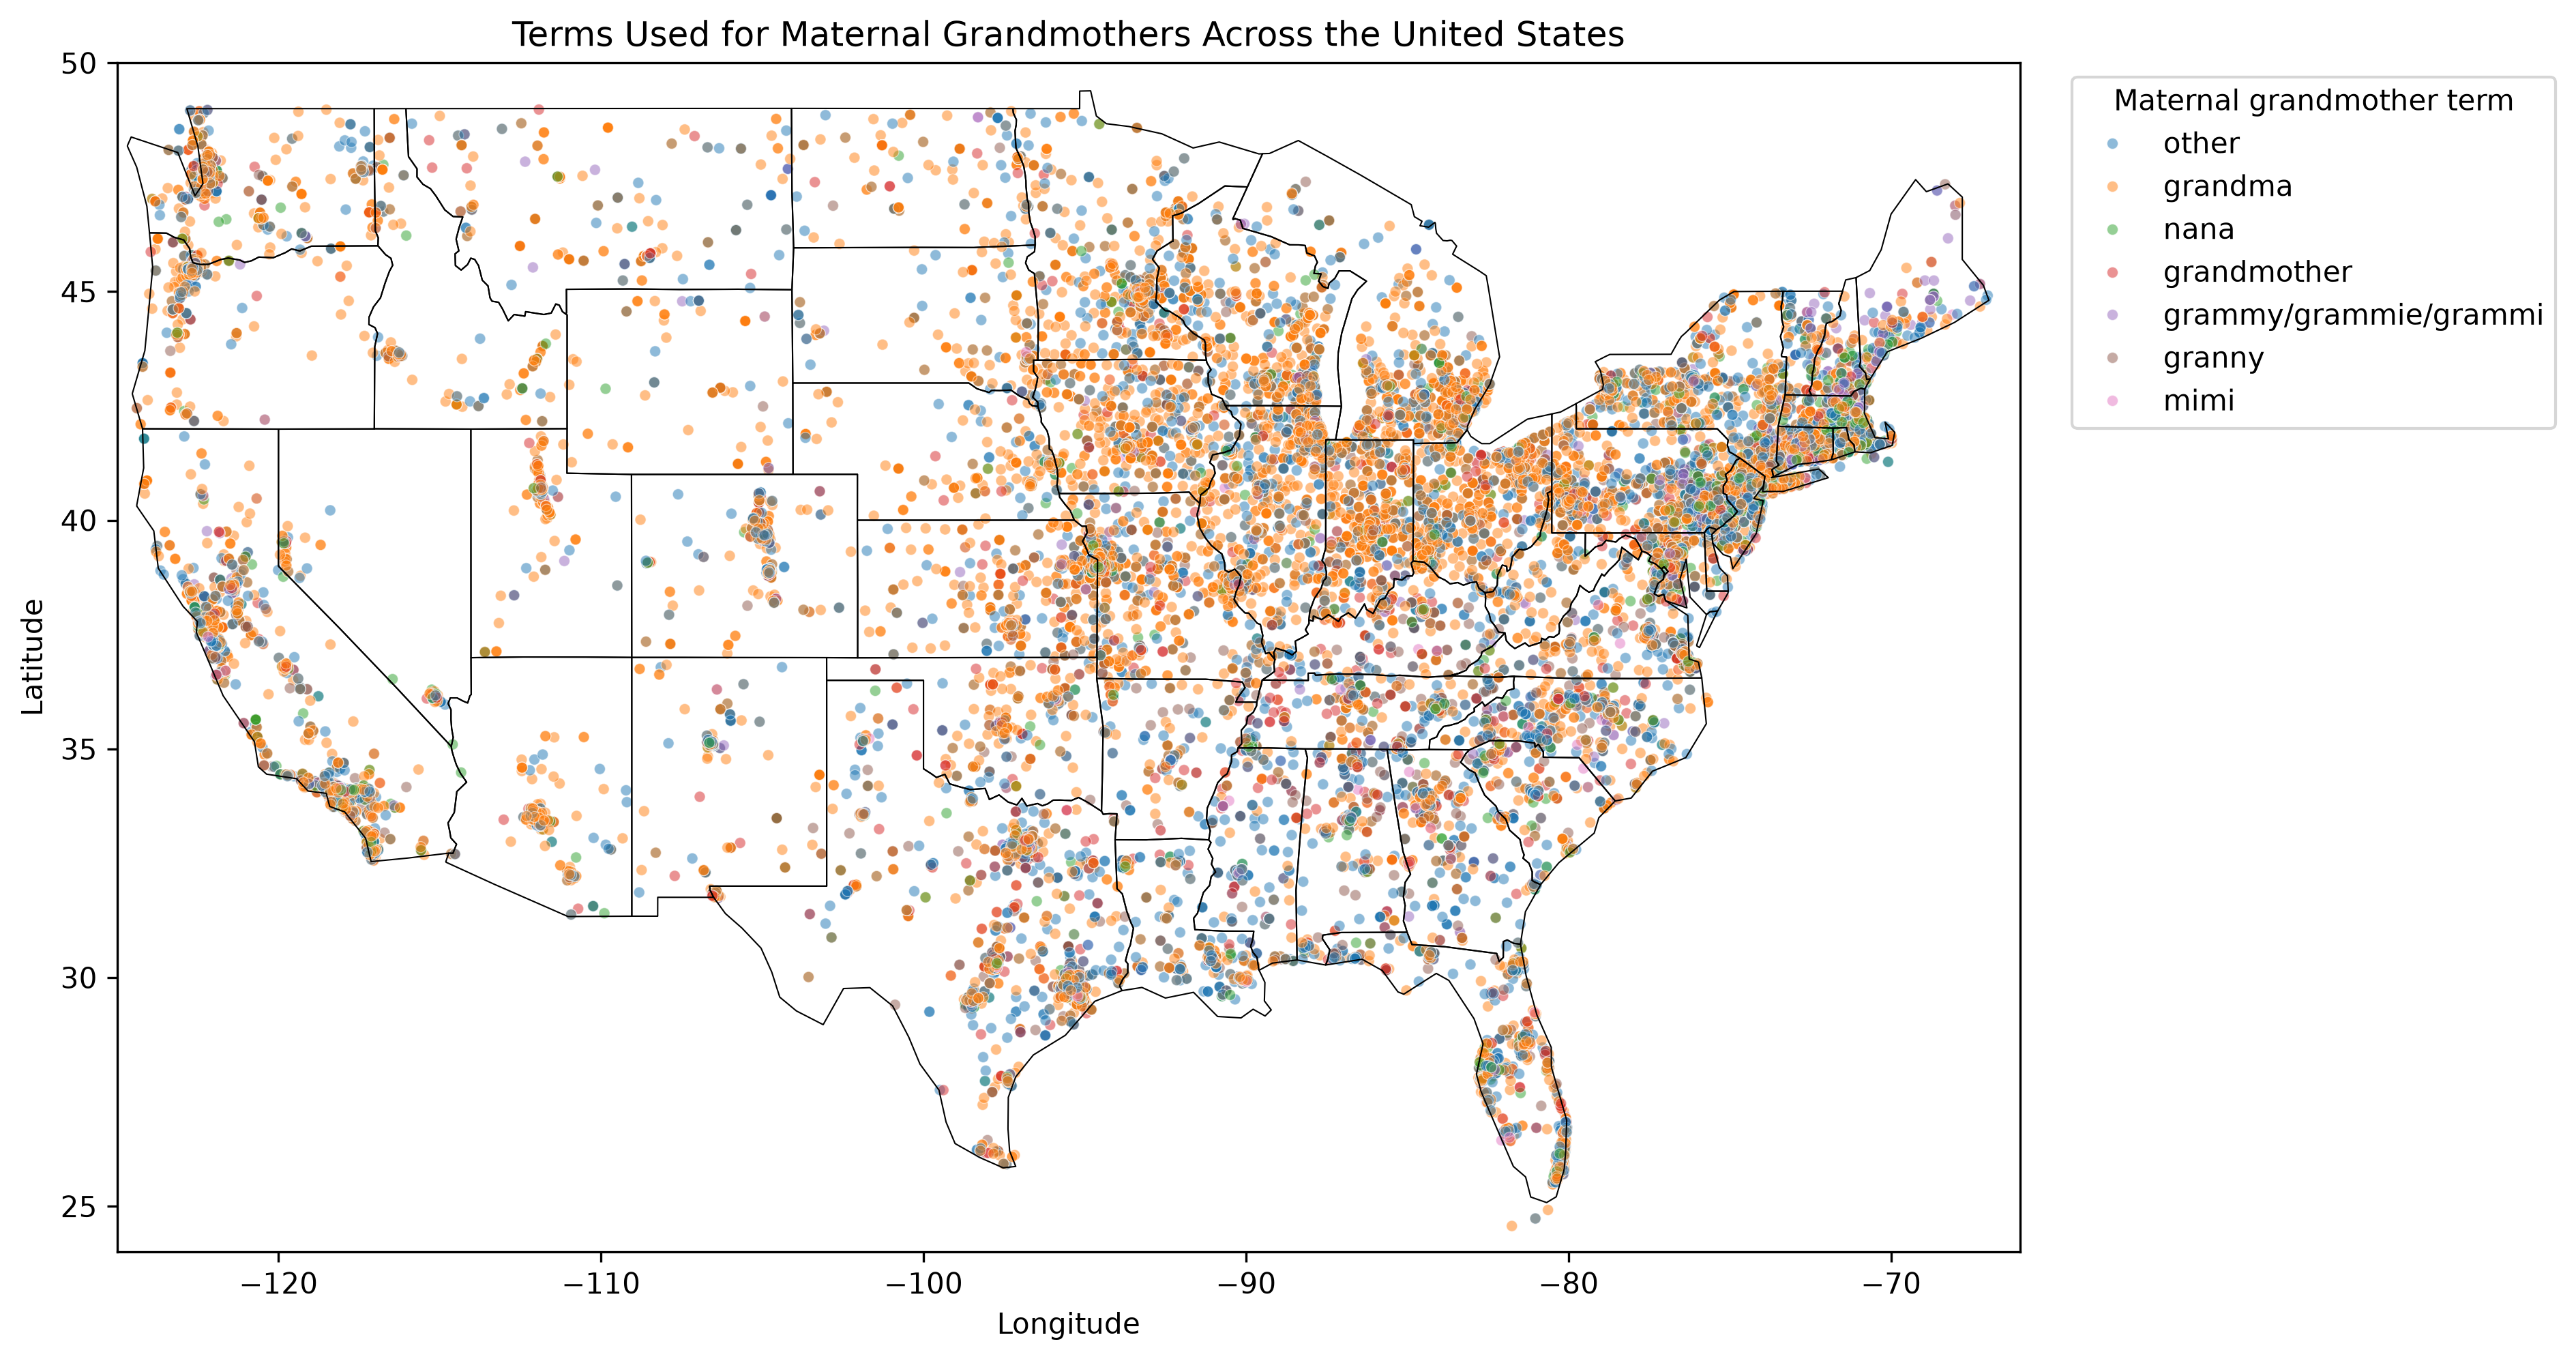
\includegraphics[keepaspectratio,alt={Geographic distribution of terms used for maternal grandmothers across the United States.}]{q68_maternal_grandmother_map.png}}
\caption{Geographic distribution of terms used for maternal grandmothers
across the United States.}
\end{figure}

\begin{figure}
\centering
\pandocbounded{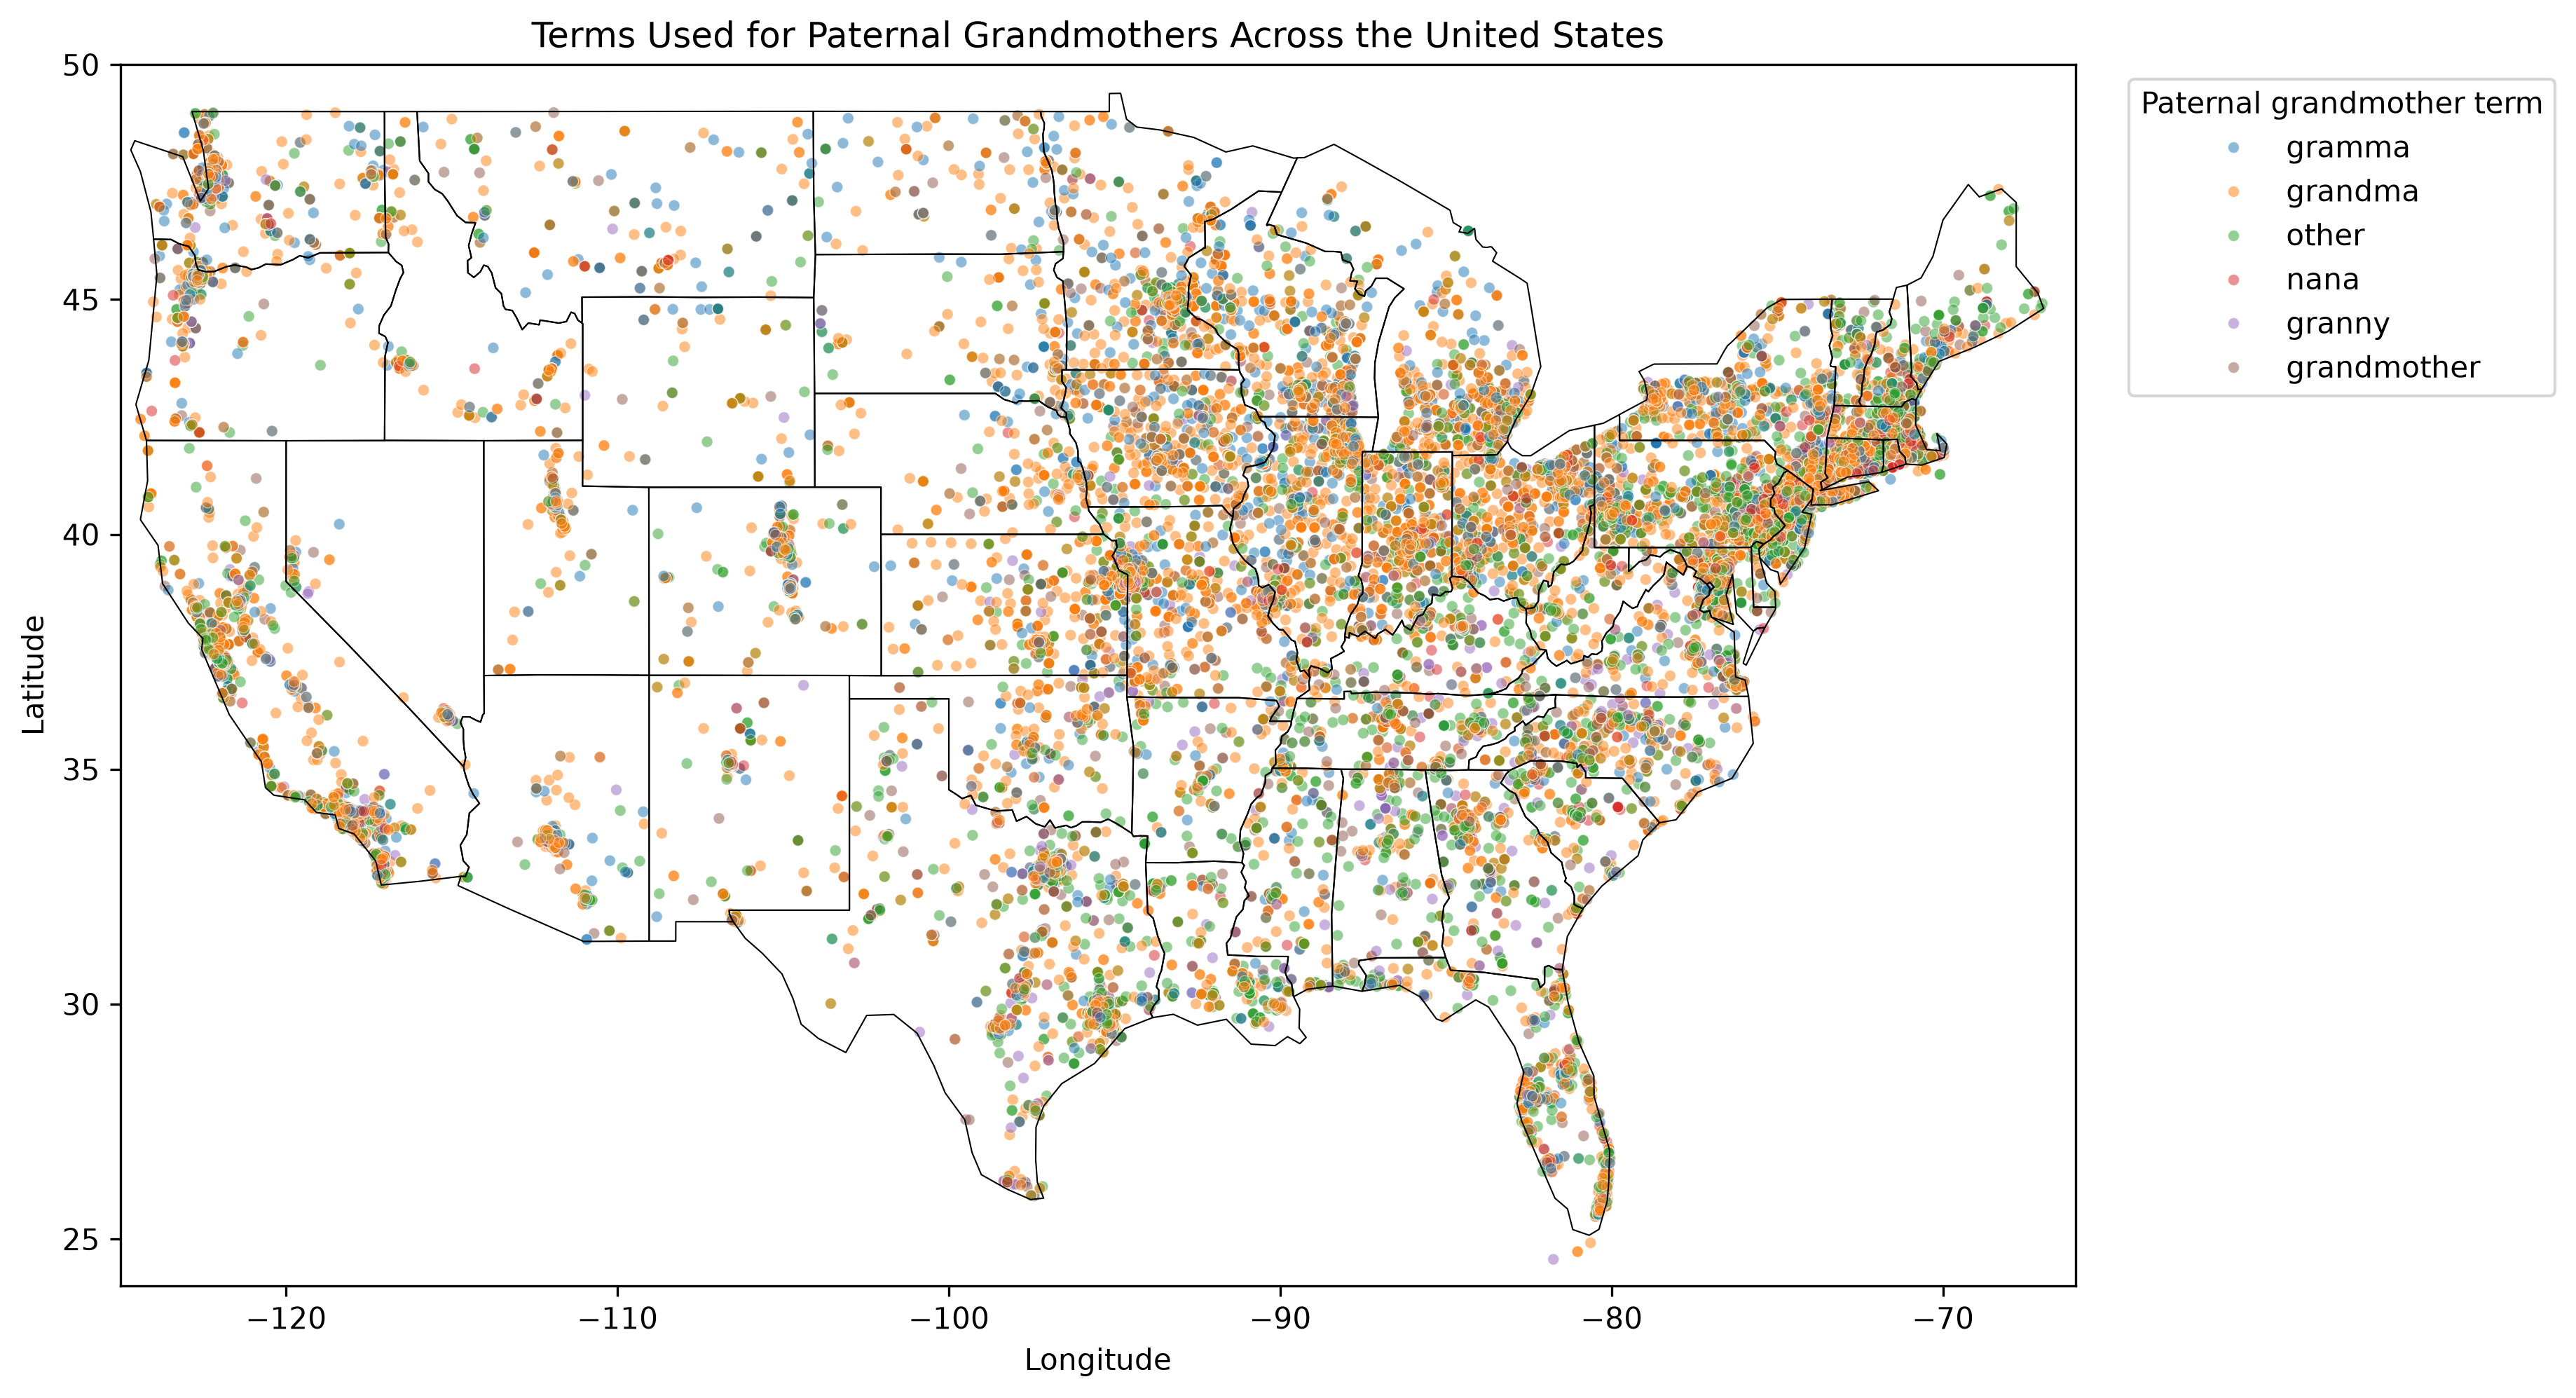
\includegraphics[keepaspectratio,alt={Geographic distribution of terms used for paternal grandmothers across the United States.}]{q69_paternal_grandmother_map.png}}
\caption{Geographic distribution of terms used for paternal grandmothers
across the United States.}
\end{figure}

The two questions were also strongly related. Among respondents who
answered both questions, 55.8\% used the same response label for their
maternal and paternal grandmothers. For example, 72.4\% of respondents
who used ``grandma'' for their maternal grandmother also used
``grandma'' for their paternal grandmother. At the state level, maternal
and paternal usage rates were highly correlated for ``granny'' (r =
0.897) and ``nana'' (r = 0.908).

I extended the analysis to Q70 and Q71, which ask about maternal and
paternal grandfather terminology. Similar geographic patterns appeared
in these questions. After harmonizing slightly different response
categories between Q70 and Q71, 65.4\% of respondents used the same term
for both grandfathers. State-level usage was also strongly correlated
for several terms, including ``grandpa'' (r = 0.879) and ``grampa'' (r =
0.898). Together, these results suggest that regional patterns in
grandparent terminology are present across multiple related linguistic
questions.

\subsection{3. Dimension Reduction}\label{dimension-reduction}

As described in the data-cleaning section, I transformed the original
categorical responses into binary variables. The initial one-hot
encoding produced 535 binary variables, and after removing the 67
indicators corresponding to nonresponses, 468 binary linguistic features
were retained. I first performed PCA using all 47,471 respondents. The
first principal component showed a noticeable geographic pattern, while
the second principal component also showed some geographic structure.
However, PC3 appeared to capture missingness rather than purely
linguistic variation: its correlation with the number of questions
answered was approximately 0.54. I therefore restricted the main PCA
analysis to the 40,061 respondents who answered all 67 questions and
repeated the analysis.

\begin{figure}
\centering
\pandocbounded{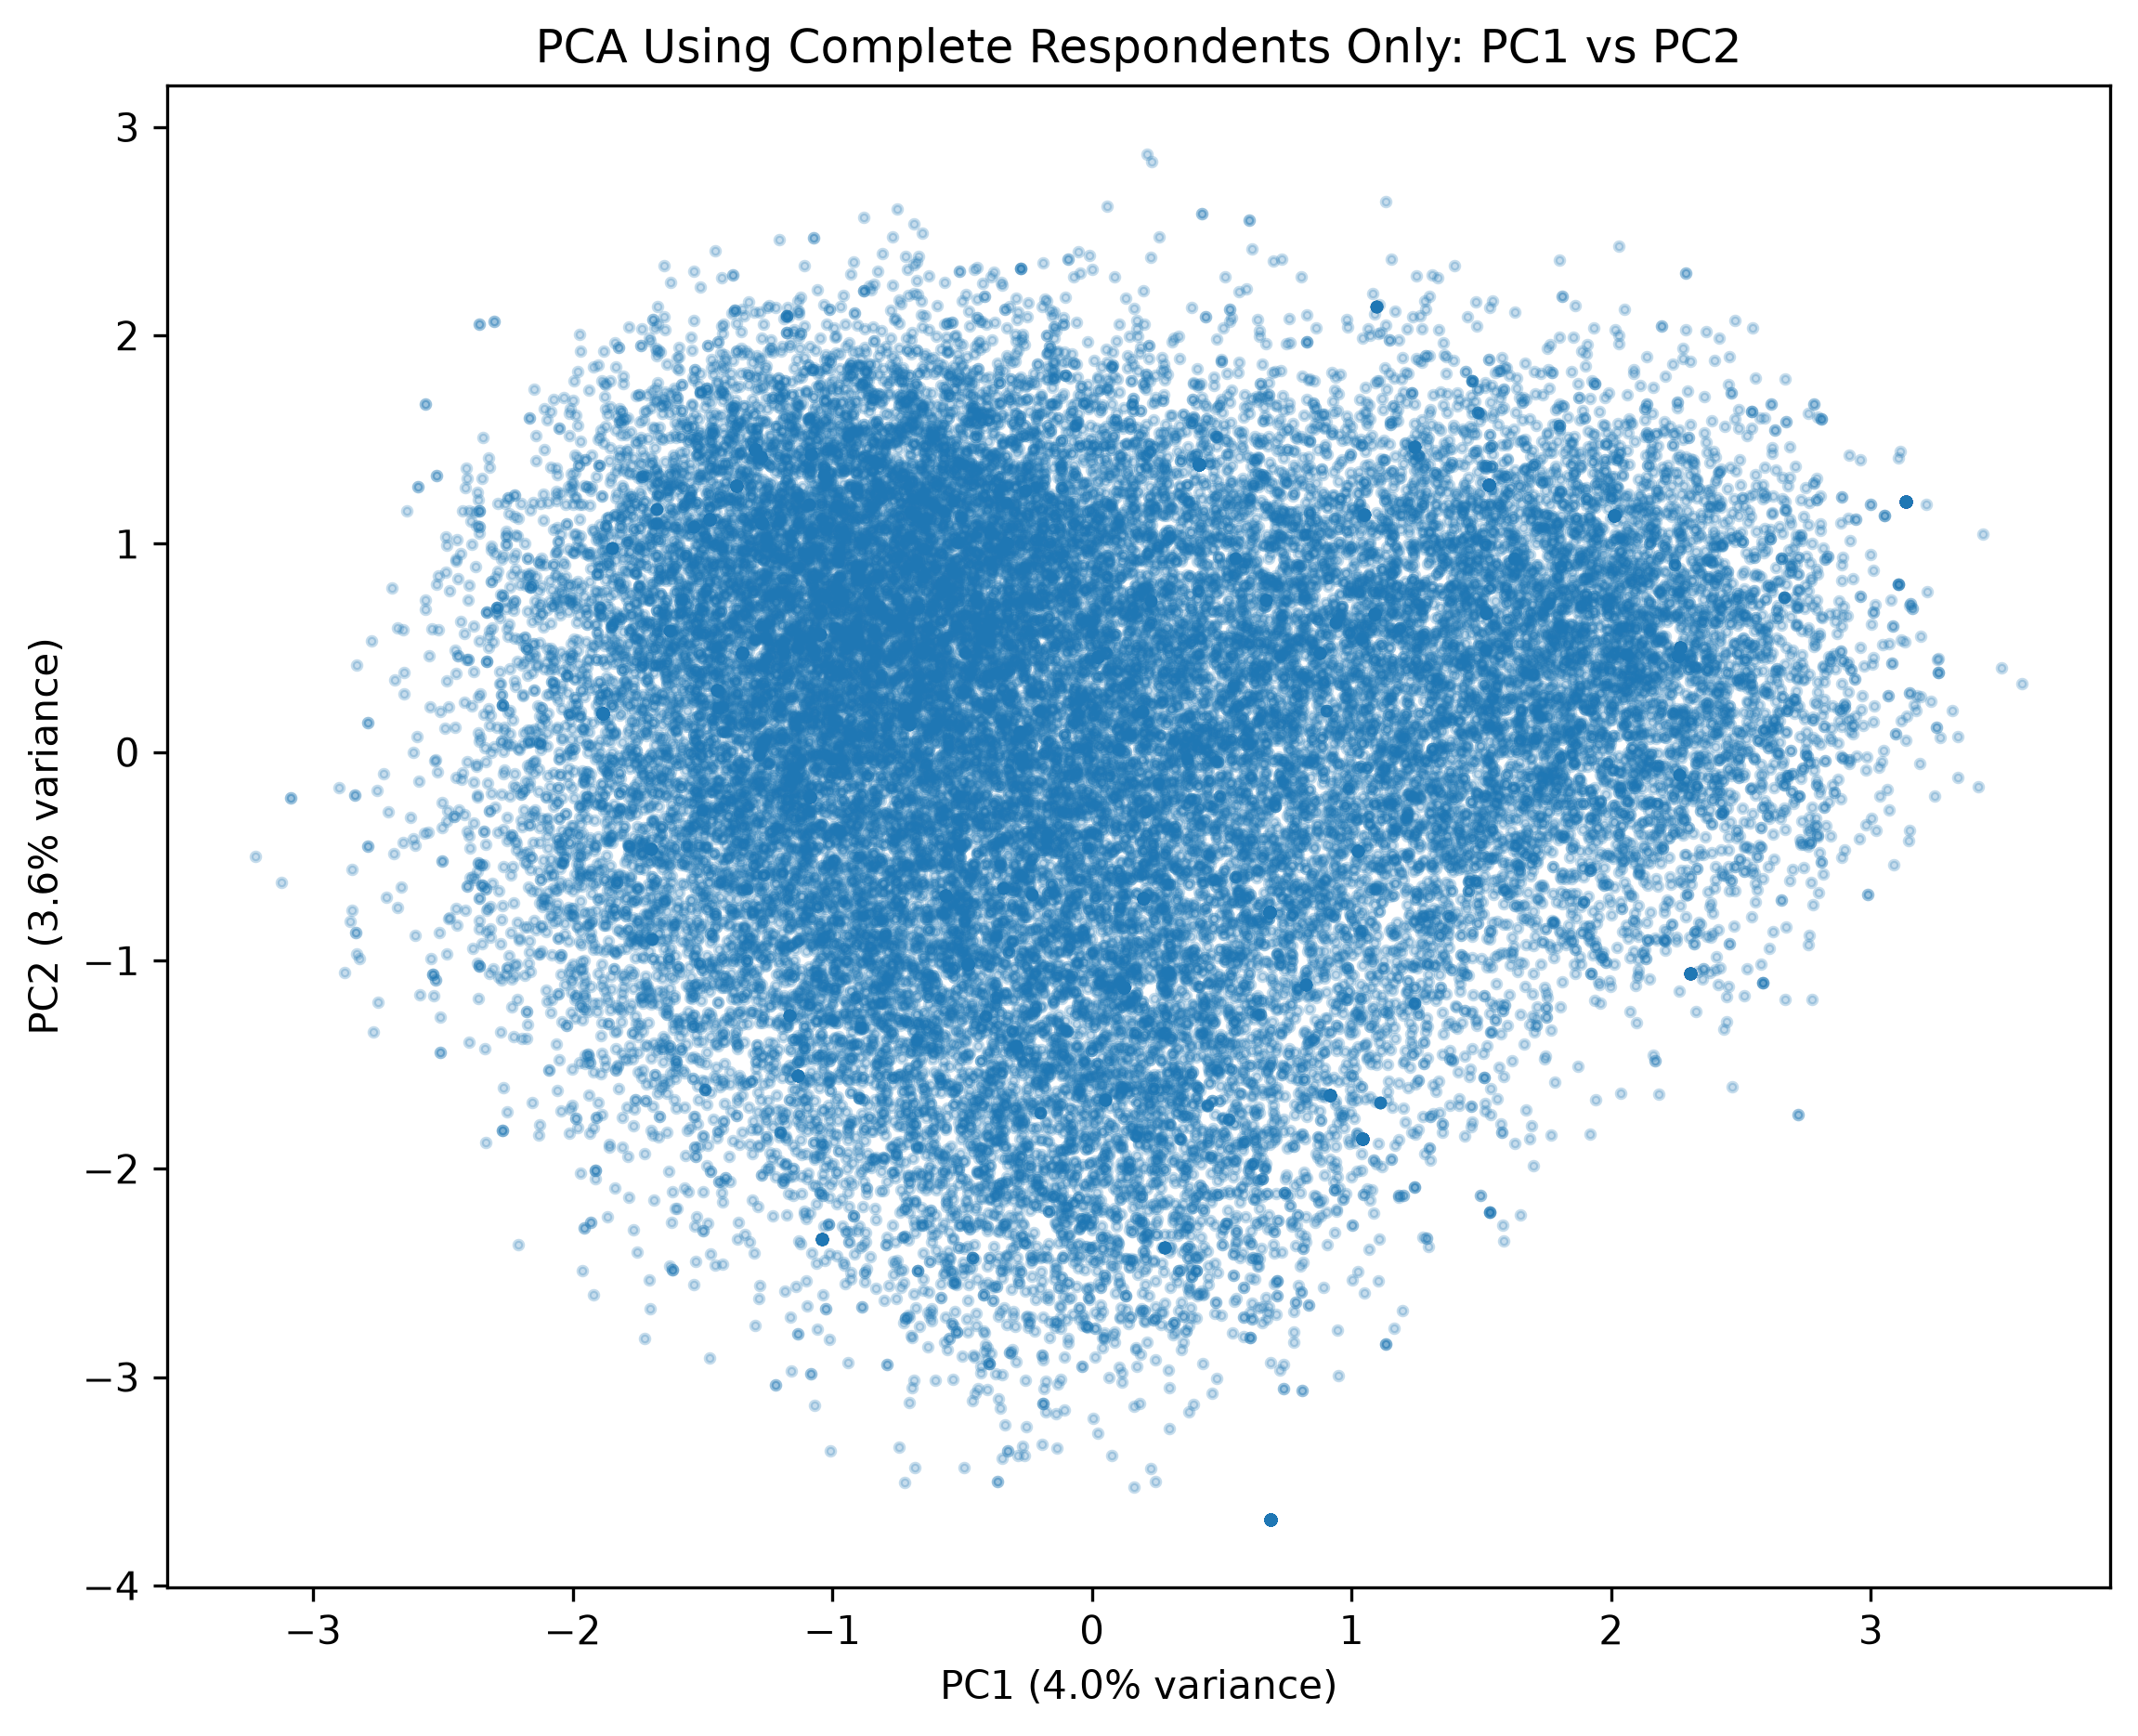
\includegraphics[keepaspectratio,alt={Projection of complete respondents onto the first two principal components.}]{pca_pc1_pc2.png}}
\caption{Projection of complete respondents onto the first two principal
components.}
\end{figure}

The PC1--PC2 projection does not show clearly separated groups of
respondents. Instead, the observations substantially overlap, suggesting
that the linguistic differences represented by the first two principal
components may be more continuous than discrete. The first two
components explain only about 7.6\% of the total variance, so this
two-dimensional projection captures only a limited portion of the
overall variation in the data.

\begin{figure}
\centering
\pandocbounded{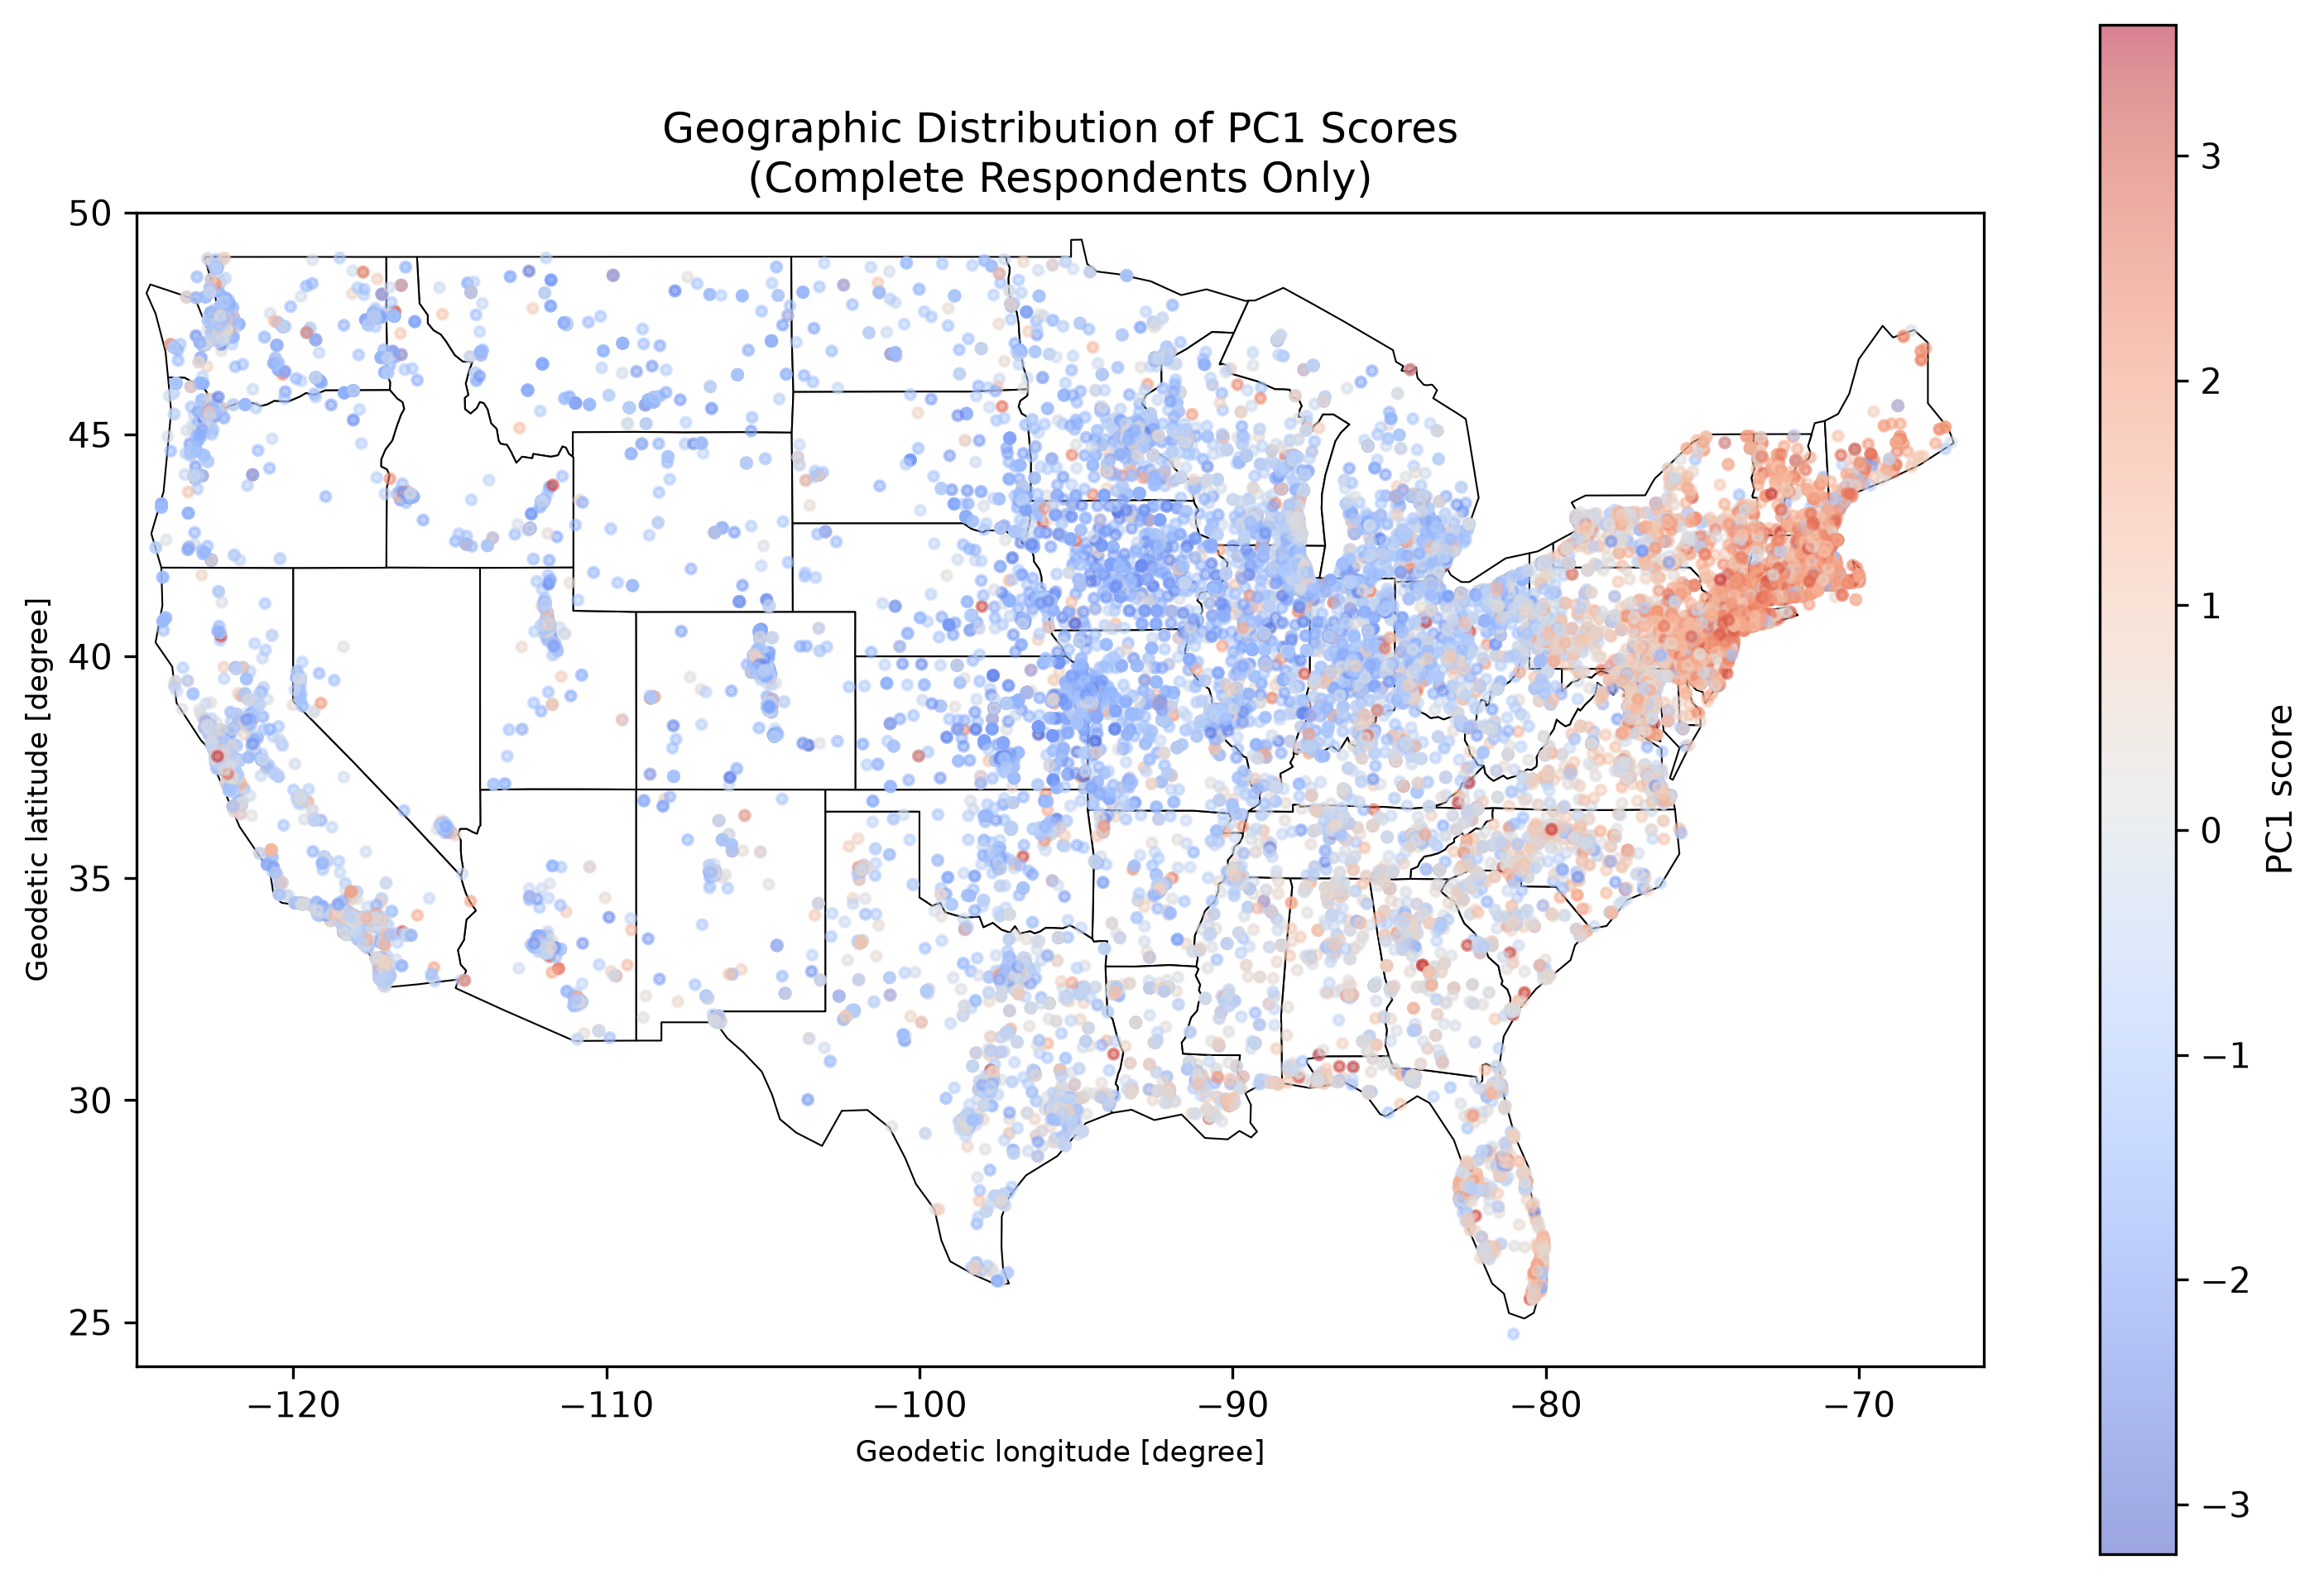
\includegraphics[keepaspectratio,alt={Geographic distribution of PC1 scores among complete respondents.}]{pca_pc1_geographic.png}}
\caption{Geographic distribution of PC1 scores among complete
respondents.}
\end{figure}

\begin{figure}
\centering
\pandocbounded{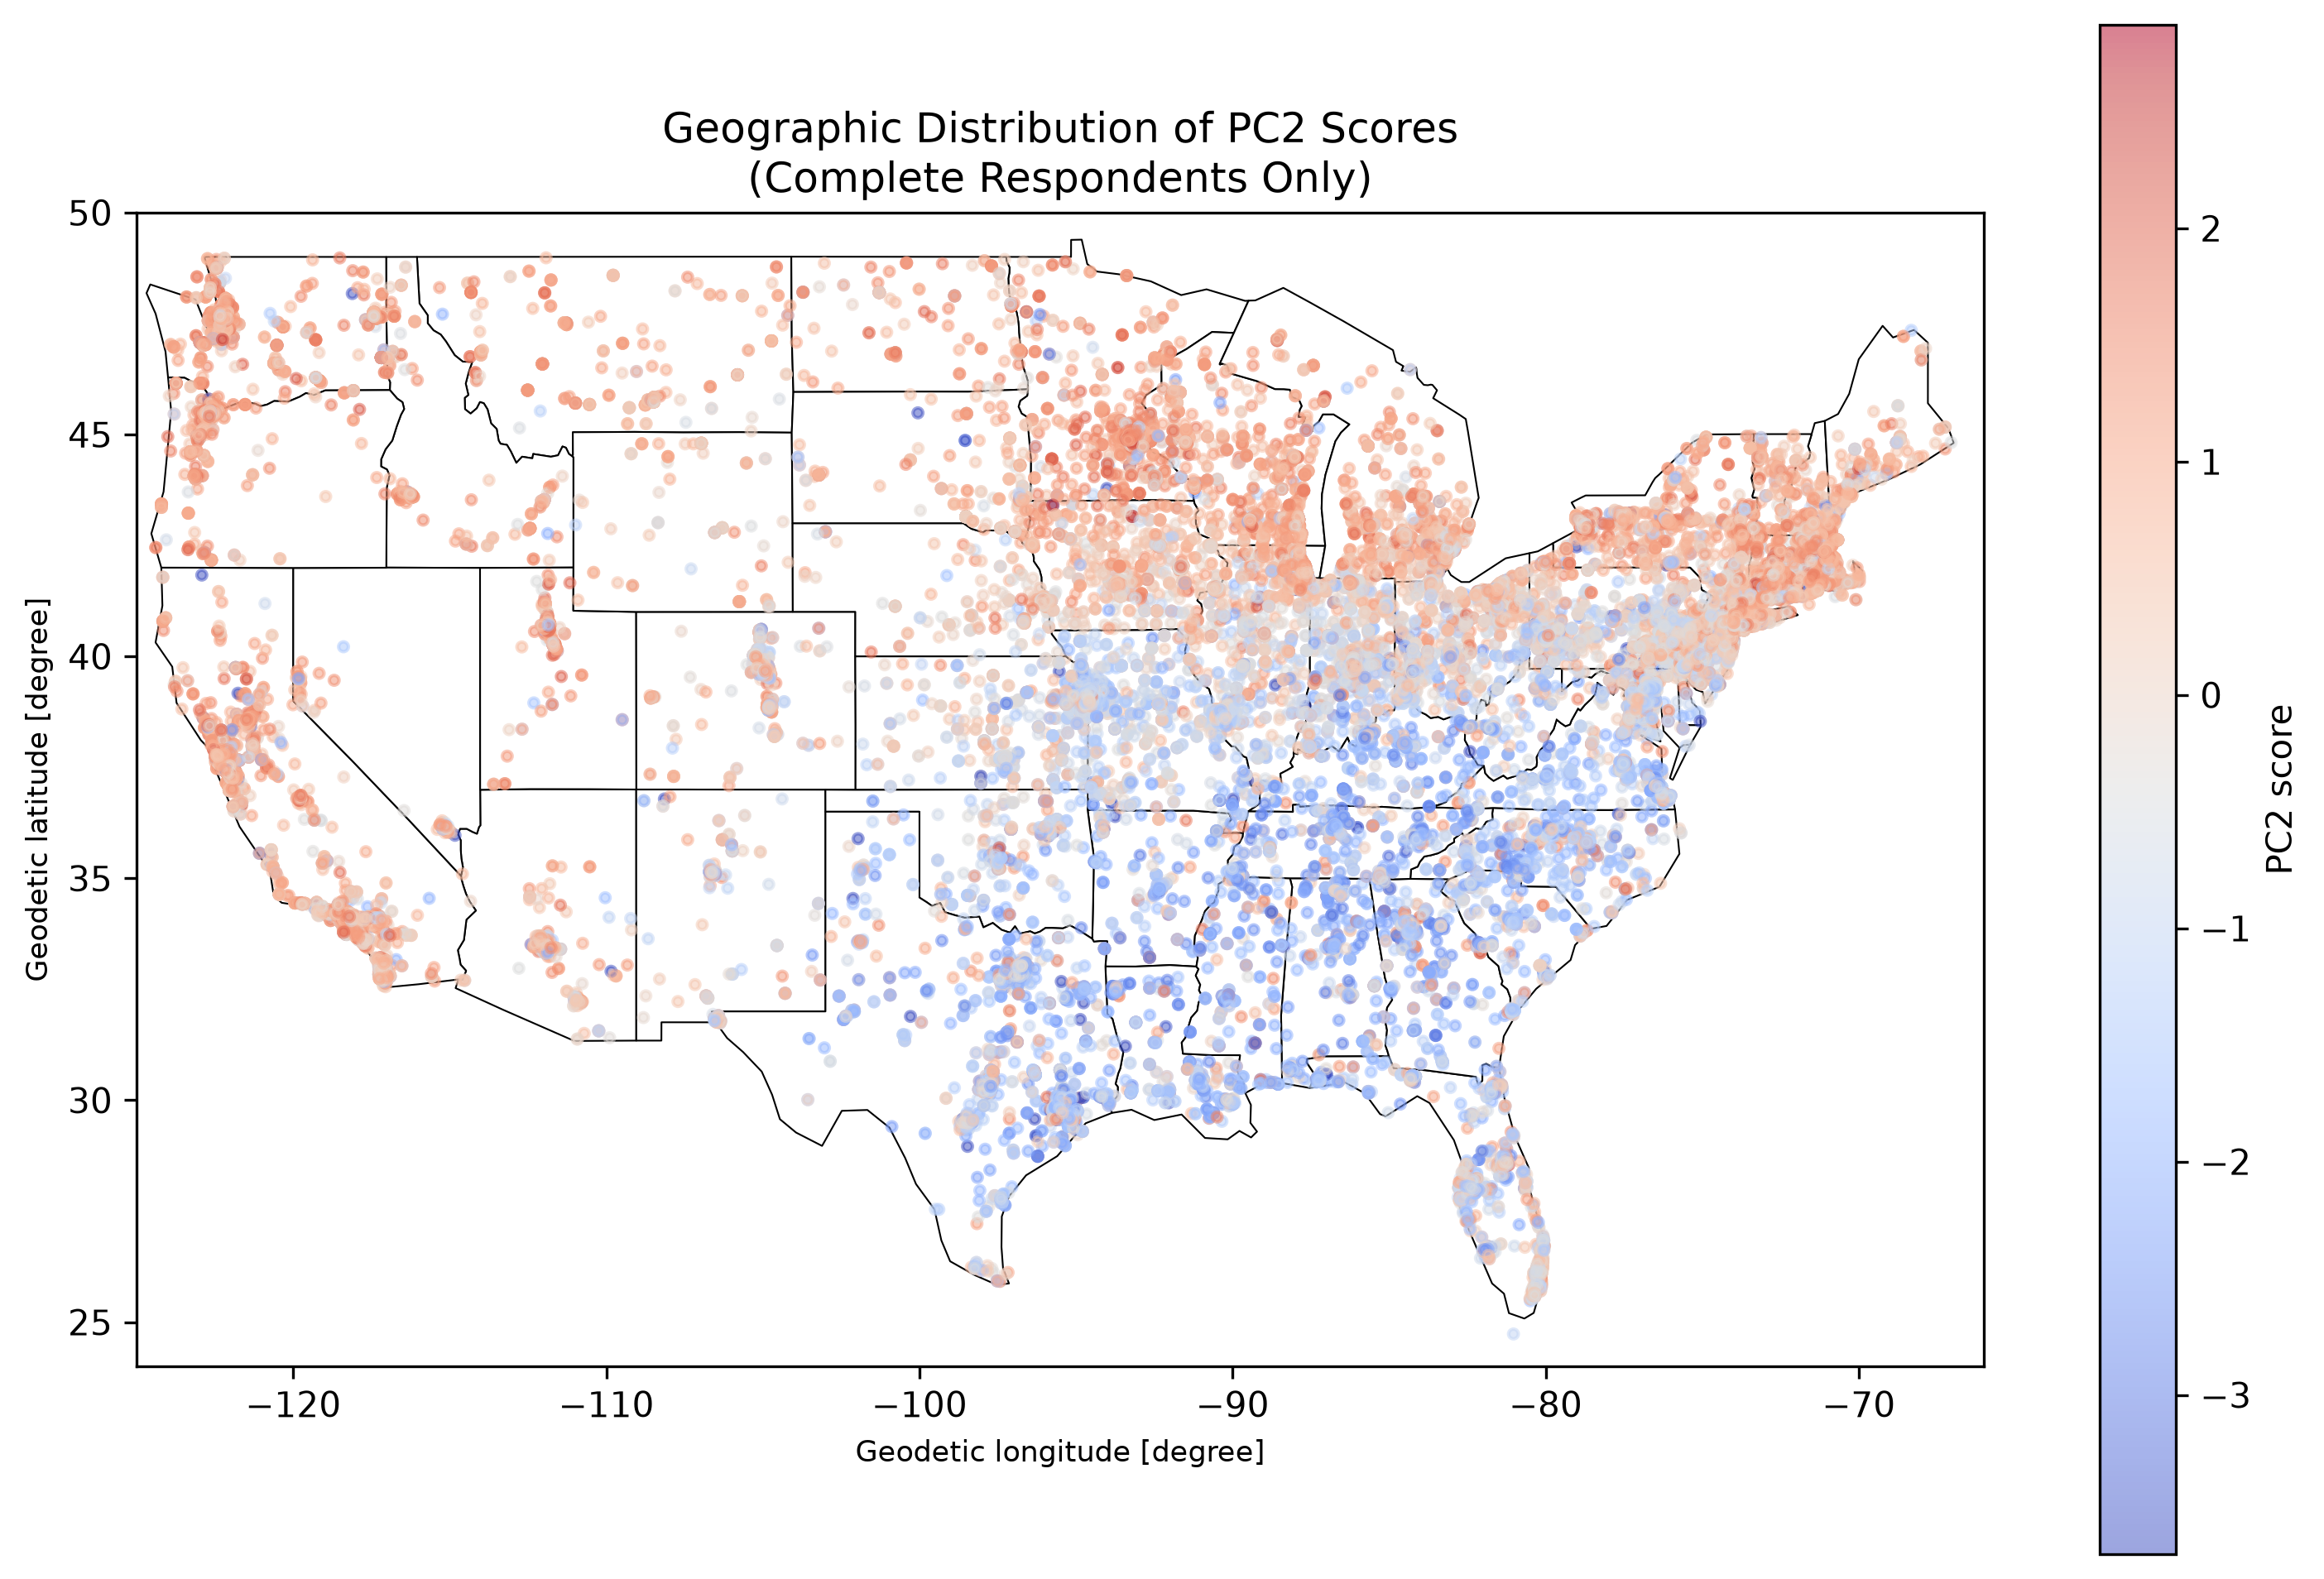
\includegraphics[keepaspectratio,alt={Geographic distribution of PC2 scores among complete respondents.}]{pca_pc2_geographic.png}}
\caption{Geographic distribution of PC2 scores among complete
respondents.}
\end{figure}

Although the PCA scatter plot does not reveal clearly separated groups,
mapping the principal component scores reveals geographic structure. PC1
in particular shows a noticeable contrast between the Northeast and much
of the interior and western United States. PC2 also exhibits geographic
variation, although its pattern is less pronounced. Thus, the PCA
suggests that some of the variation in responses is geographically
structured even though respondents do not form clearly separated groups
in the low-dimensional projection.

The binary features were centered but not standardized. Scikit-learn's
PCA centers each feature by default. I did not scale the features to
unit variance because all features were binary indicators on the same
0--1 scale. Standardizing these indicators would give relatively greater
weight to rare response categories, which I did not want to emphasize
disproportionately in the PCA.

I did not apply PCA directly to the original categorical response codes
because the numerical codes are arbitrary category labels rather than
quantitative measurements. Treating them as numerical values would
impose artificial ordering and distances between response categories.
Binary encoding avoids imposing this numerical structure.

\subsection{4. Clustering}\label{clustering}

I used two clustering methods, K-means and spectral clustering. For
K-means, I analyzed the 40,061 respondents who answered all 67 survey
questions using the 468 binary linguistic features described above. I
compared solutions from k=2 to k=10. The elbow plot did not show a clear
cutoff, but the silhouette score was highest at k=3, with a value of
approximately 0.032. Based on this result, I selected three clusters for
the main K-means analysis. The three clusters contained 11,433, 11,406,
and 17,222 respondents, respectively. However, the silhouette score was
very low even at its maximum, suggesting substantial overlap between the
clusters. Therefore, the three clusters should not be interpreted as
three clearly separated or objectively distinct linguistic populations.

\begin{figure}
\centering
\pandocbounded{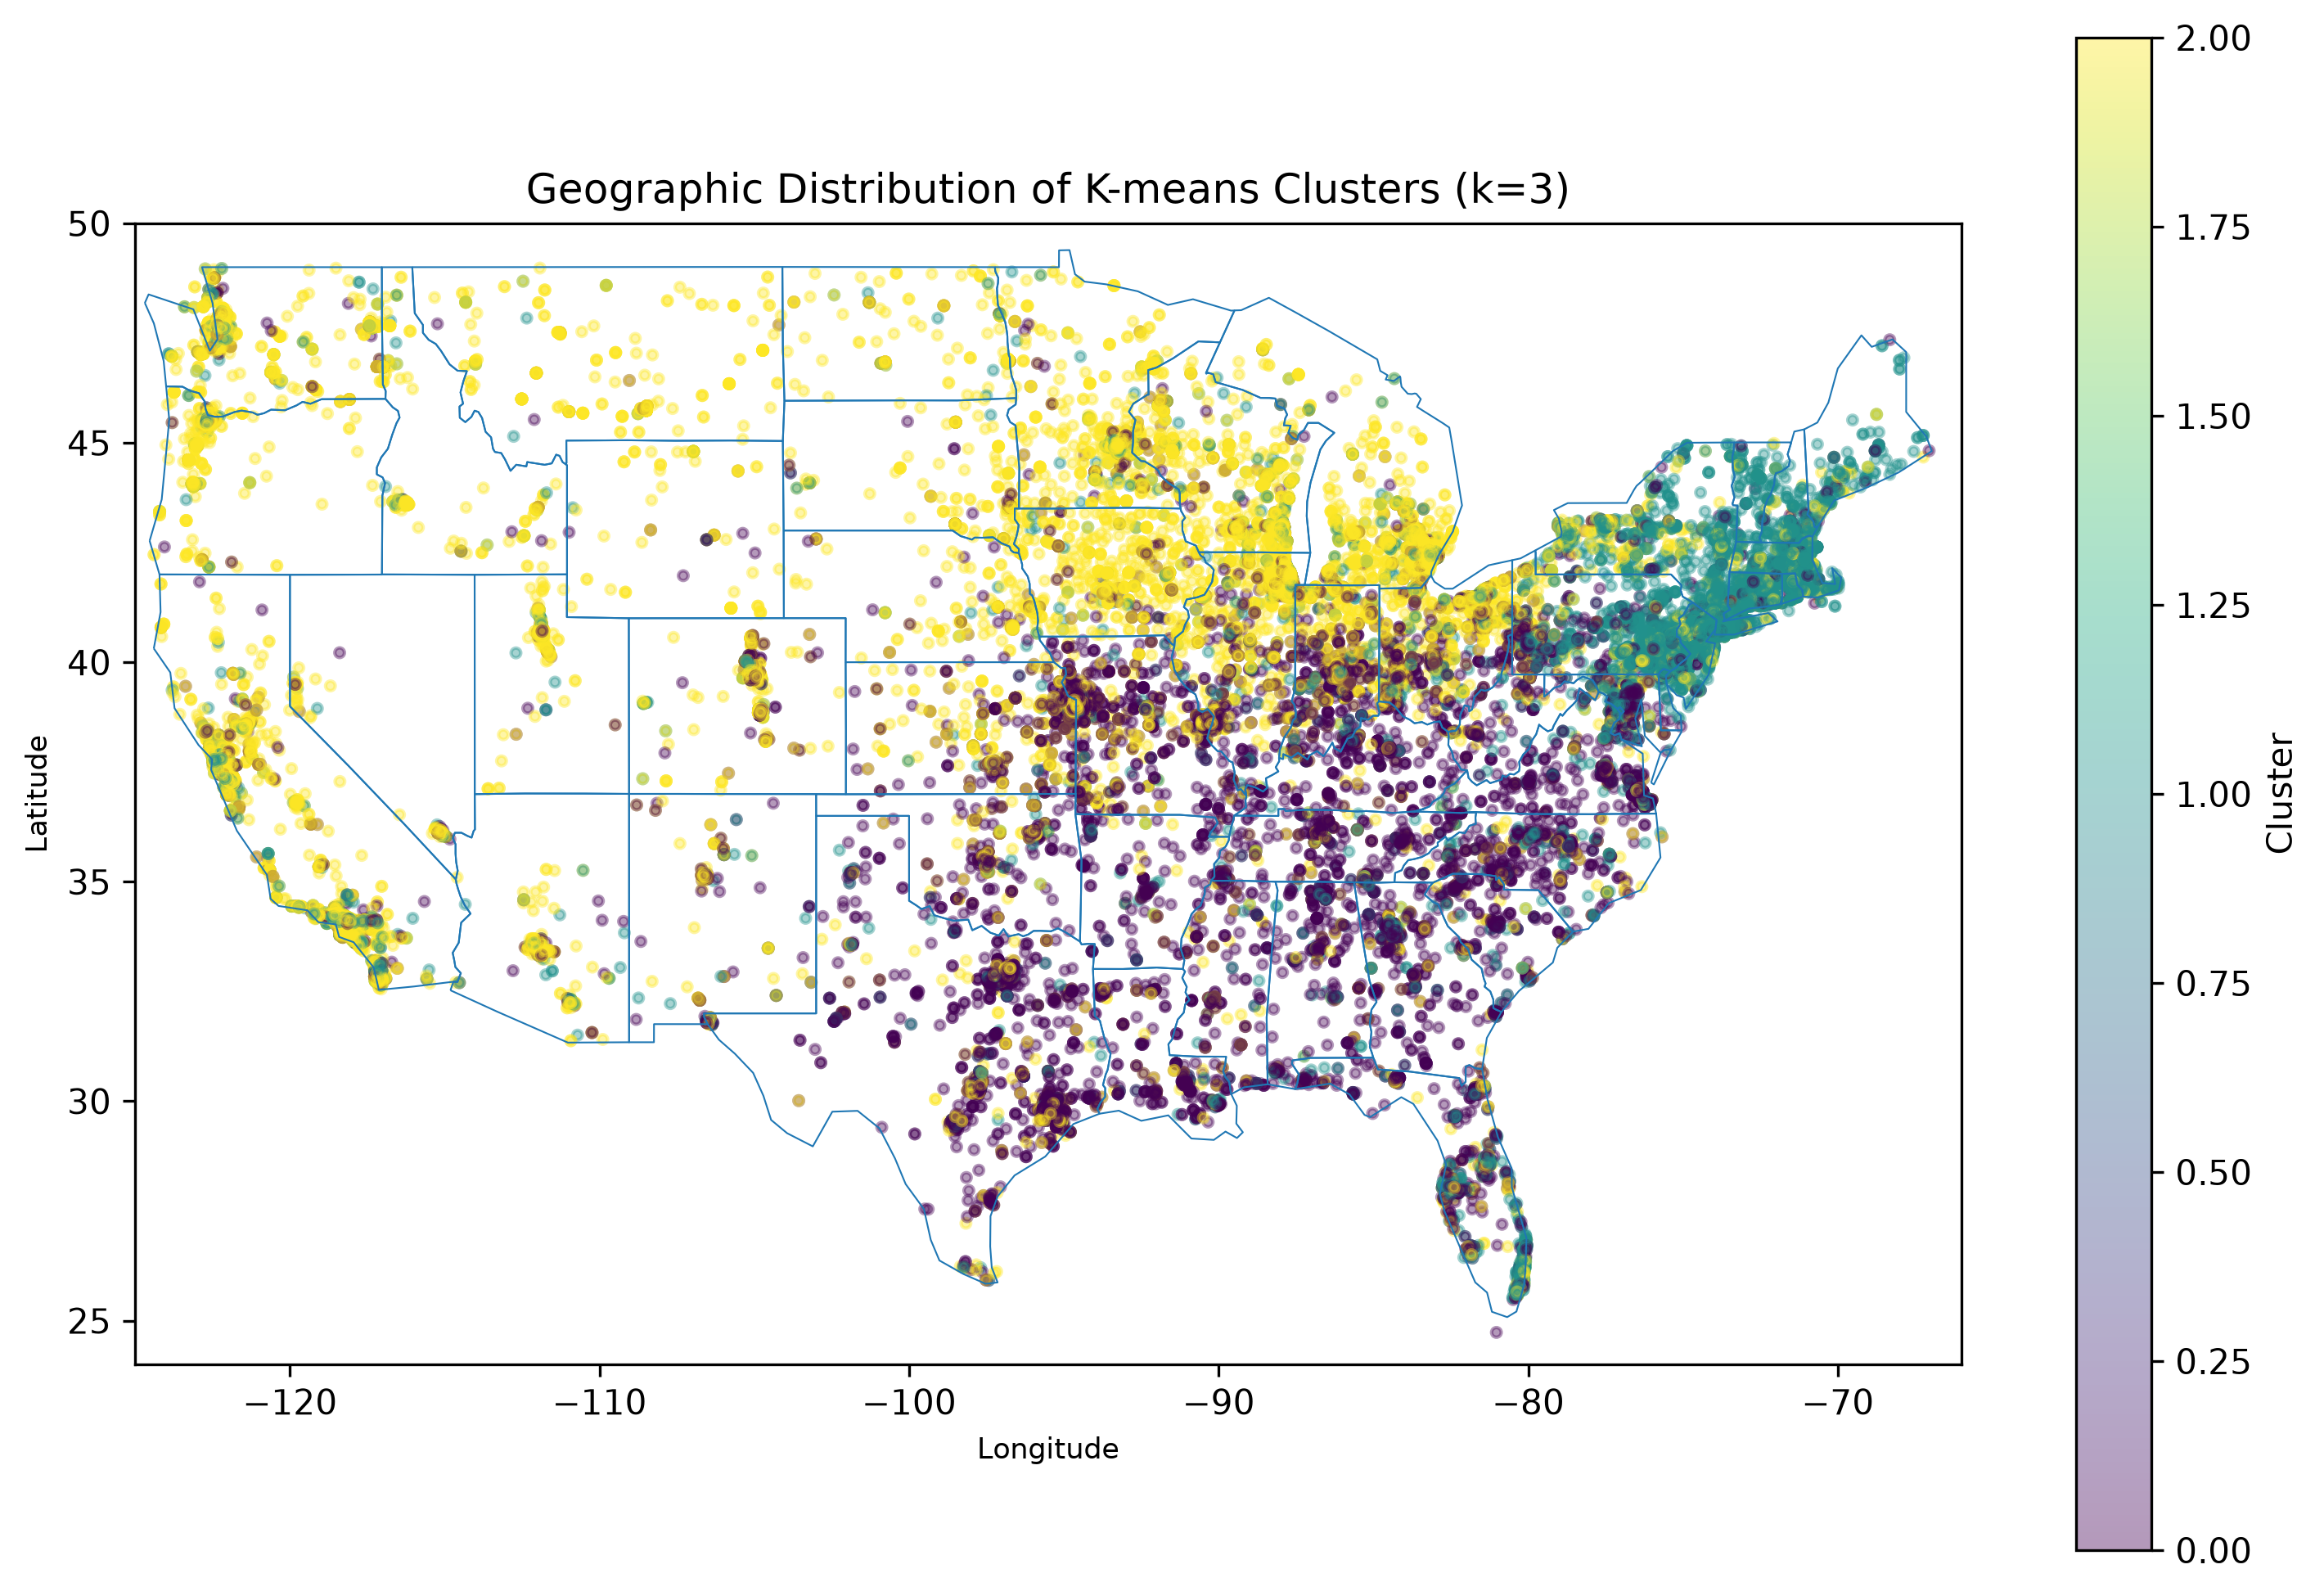
\includegraphics[keepaspectratio,alt={Geographic distribution of the three K-means clusters among complete respondents.}]{kmeans_clusters_map.png}}
\caption{Geographic distribution of the three K-means clusters among
complete respondents.}
\end{figure}

Despite the substantial overlap, the K-means clusters showed clear
geographic structure when mapped across the United States. The three
clusters roughly corresponded to the Northeast, the South/interior, and
the North/West/Upper Midwest, although there was considerable geographic
mixing near their boundaries. Several linguistic responses also strongly
distinguished the clusters. For example, ``sneakers'' was used by 88.8\%
of respondents in Cluster 1, compared with only about 15--17\% in the
other two clusters. ``Y'all'' was much more common in Cluster 0
(51.1\%), while ``pop'' was most common in Cluster 2 (52.0\%). In
contrast, ``soda'' was especially common in Cluster 1 (84.3\%). Other
differences, such as ``kitty-corner'' versus ``catty-corner'' and
``drinking fountain'' versus ``water fountain,'' also contributed to the
separation of the clusters. These patterns suggest that the clusters
capture meaningful regional differences in lexical usage, even though
their boundaries are not sharply separated.

\begin{figure}
\centering
\pandocbounded{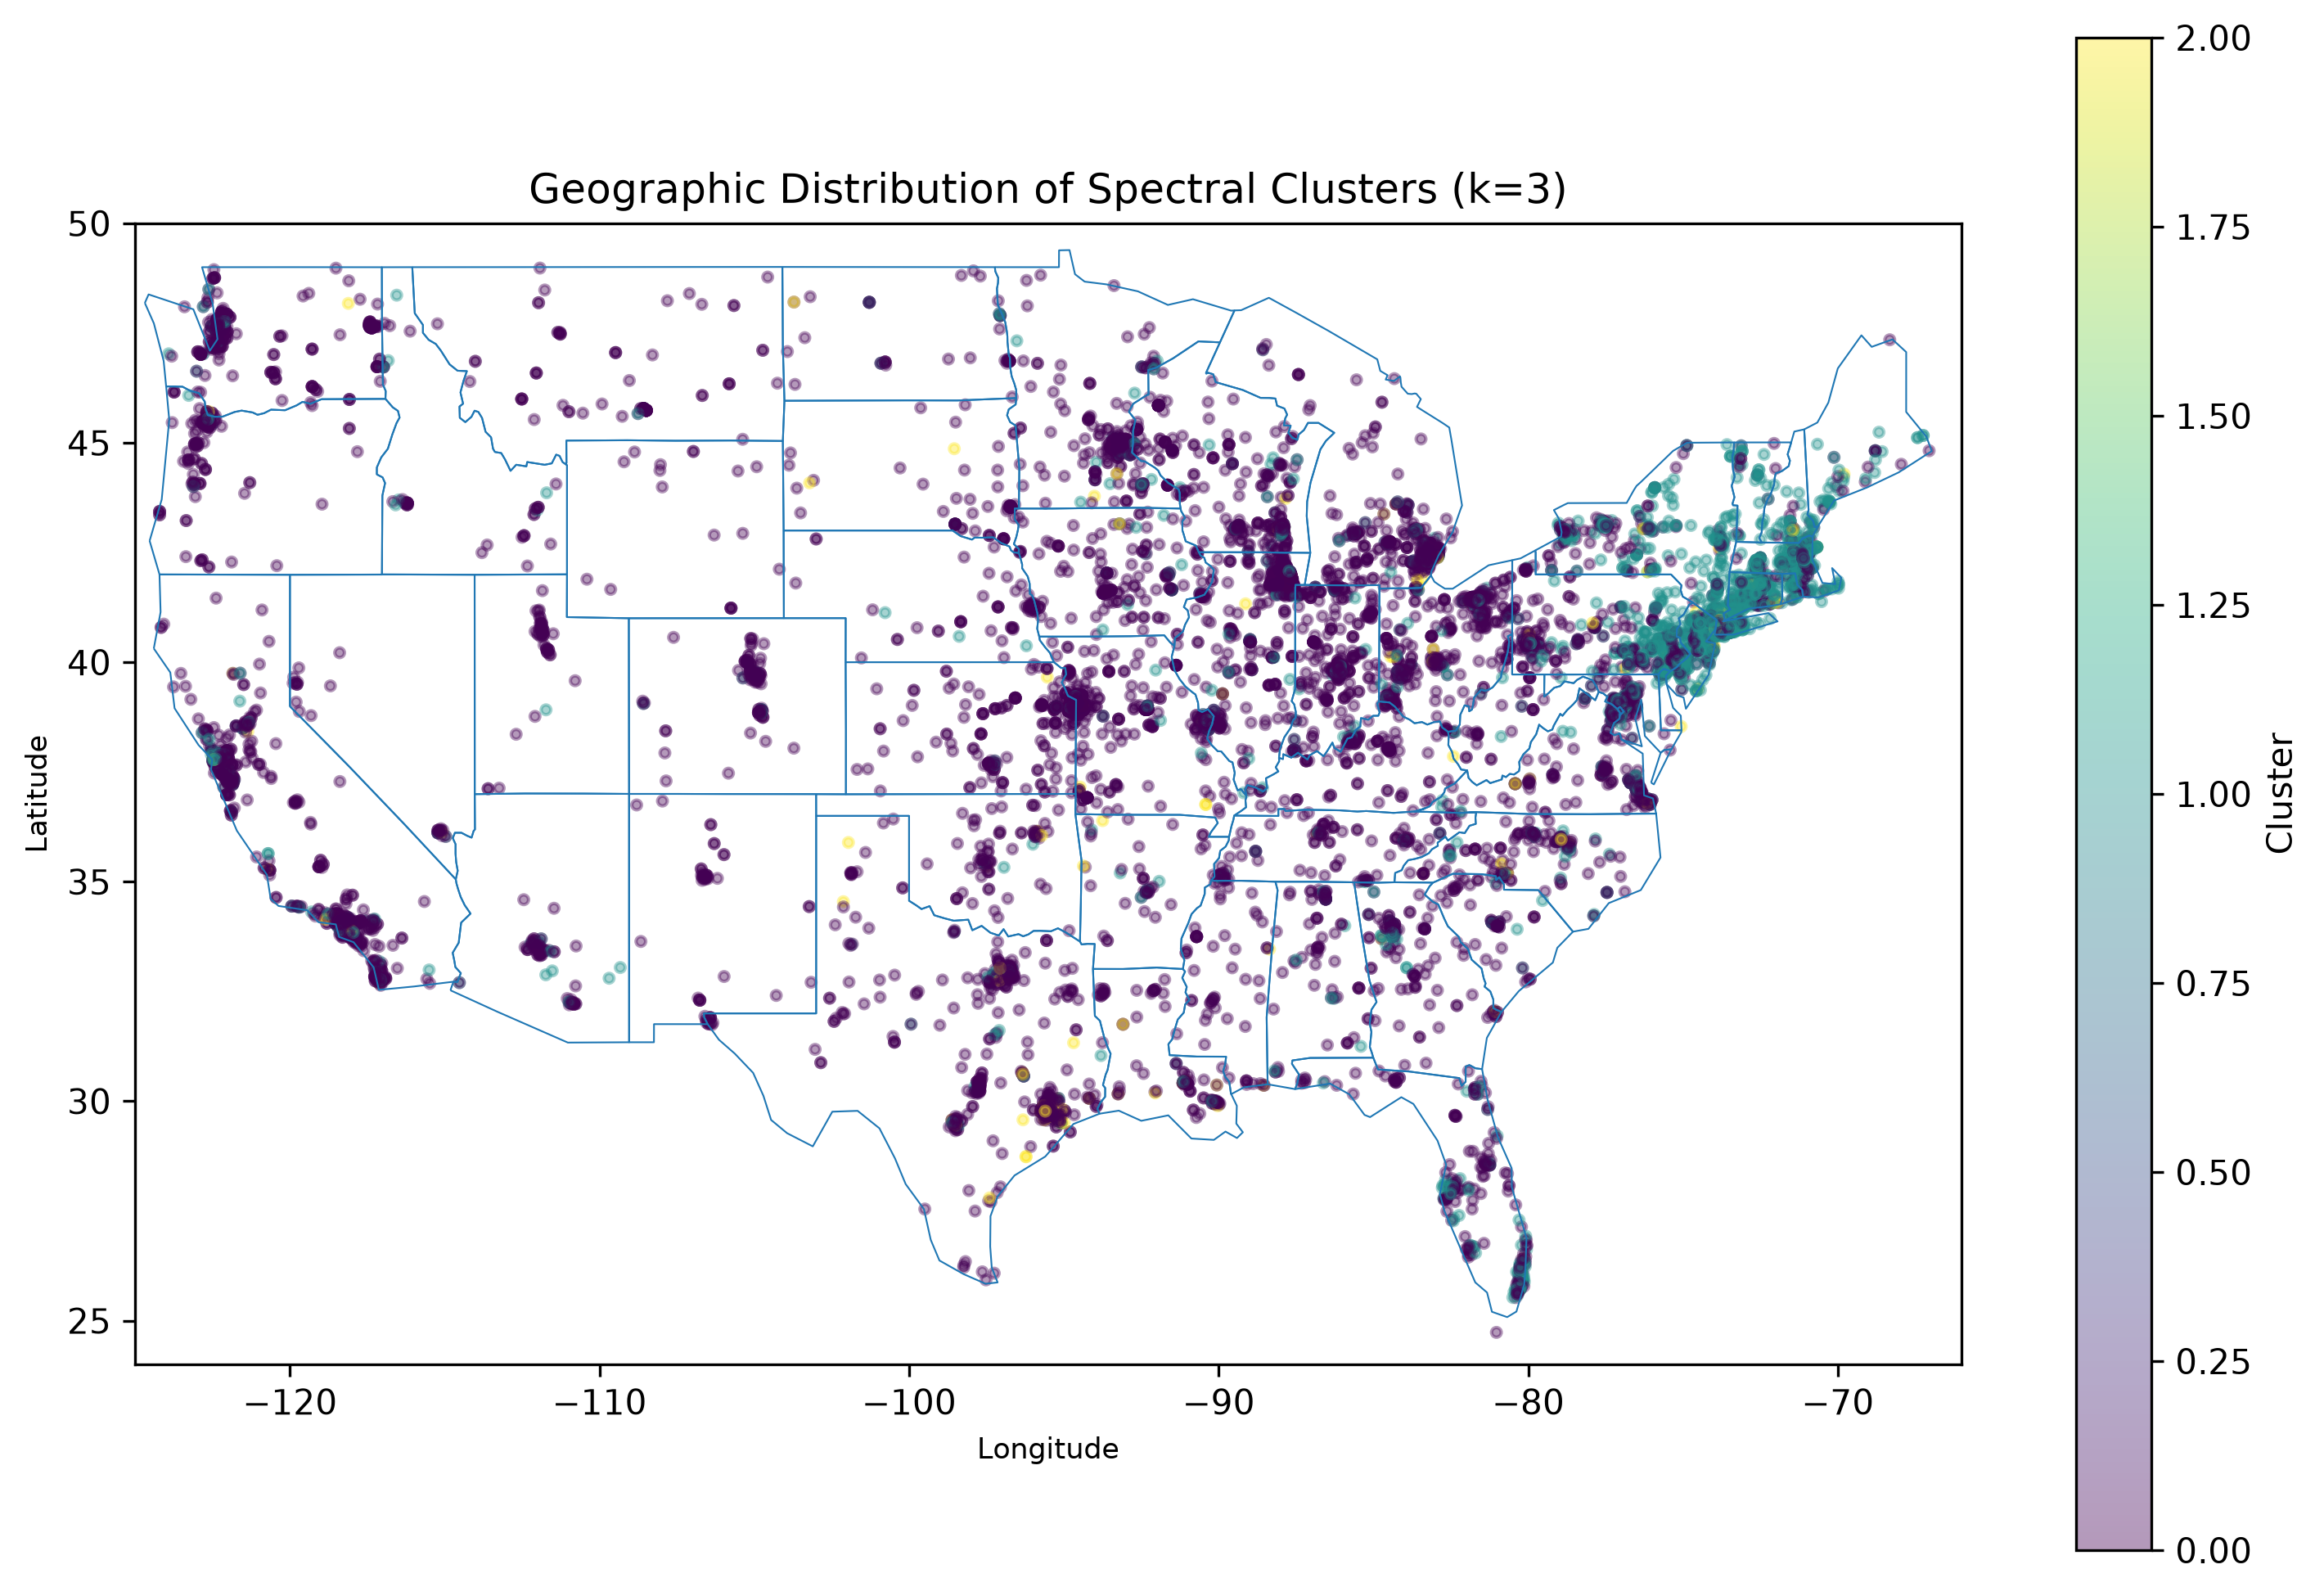
\includegraphics[keepaspectratio,alt={Geographic distribution of the three spectral clusters in the 10,000-respondent subsample.}]{spectral_clusters_map.png}}
\caption{Geographic distribution of the three spectral clusters in the
10,000-respondent subsample.}
\end{figure}

For spectral clustering, I used a random sample of 10,000 complete
respondents because applying the method to the full dataset was
computationally expensive. I performed the analysis using the first 10
PCA coordinates. With n\_neighbors=10, the similarity graph was
disconnected and produced an uninformative clustering result. I
therefore examined graph connectivity using different values of
n\_neighbors. The graph became fully connected at n\_neighbors=200, so I
used this value for the final spectral clustering analysis.

I used k=3 for spectral clustering primarily to make the results
directly comparable with the three-cluster K-means solution. The
eigenvalue gaps did not provide strong evidence for exactly three
spectral clusters, so k=3 should not be interpreted as a uniquely
supported number of clusters for this method.

The spectral clustering result differed substantially from the K-means
solution. One spectral cluster captured the Northeast in a way that was
quite similar to the corresponding K-means cluster. However, spectral
clustering combined most of the remaining respondents into one large
cluster and separated a much smaller cluster containing only 177
respondents. The overall agreement between the two methods was moderate,
with an Adjusted Rand Index (ARI) of approximately 0.387 and a
Normalized Mutual Information (NMI) of approximately 0.510. Thus, the
two methods identified some common geographic structure, particularly in
the Northeast, but did not produce the same overall partition of
respondents.

The two methods also have different advantages and limitations for these
data. K-means is computationally efficient and produces clusters that
are relatively easy to interpret, but it relies on Euclidean distance
and centroid-based separation, which may not fully represent the
structure of binary linguistic features. Spectral clustering can capture
more complex, nonlinear structures through a similarity graph, but it is
substantially more computationally expensive and, in this analysis, was
sensitive to the choice of the number of neighbors. Overall, the
geographic patterns and differences in lexical responses provide
evidence of regional linguistic structure, but the low silhouette scores
and the differences between K-means and spectral clustering suggest that
this structure is not composed of sharply separated groups. Instead, the
results are more consistent with overlapping or continuous linguistic
variation across regions.

\subsection{5. Stability of Findings to
Perturbation}\label{stability-of-findings-to-perturbation}

I evaluated the stability of the K-means clustering results in two ways.
First, I repeated K-means using different random initializations. The
resulting cluster assignments were nearly identical to the original
solution, with ARI values ranging from approximately 0.991 to 0.997.
This suggests that the K-means result is not sensitive to random
initialization.

Second, I repeatedly selected random 80\% subsamples of the complete
respondents and compared their cluster assignments with those from the
full-sample K-means solution. Across 10 repetitions, the ARI ranged from
approximately 0.984 to 0.993, with a mean of 0.988. This indicates that
the K-means solution is also highly stable to moderate changes in the
sample.

However, this stability does not imply that three clusters are the
uniquely correct representation of the data. As discussed above, the low
silhouette score and the differences between K-means and spectral
clustering suggest that the underlying linguistic variation may still be
overlapping and continuous.

\subsection{6. Conclusion}\label{conclusion}

This analysis shows that lexical variation in the United States has
meaningful geographic structure, although the boundaries between
linguistic groups are not clearly discrete. PCA revealed geographic
patterns while also showing substantial overlap among respondents, and
K-means identified three geographically interpretable clusters. However,
the low silhouette score and differences between K-means and spectral
clustering suggest that linguistic variation is better understood as
overlapping patterns rather than three clearly separated populations.

These patterns may be useful for future linguistic research and language
technologies by documenting how word choices differ across regions and
individuals. As a reality check, the geographic patterns identified here
could be compared with independently documented patterns of American
regional dialects. With more time and computational resources, I would
also apply spectral clustering to the full dataset rather than the
10,000-person subsample. Additional demographic information, such as
age, race or ethnicity, gender, and income, could also help examine how
linguistic variation is associated with individual characteristics
beyond geography.

\subsection{7. Academic Honesty}\label{academic-honesty}

\subsubsection{7.1 Statement}\label{statement}

I declare that this report represents my original work completed for
this course. All data processing, model implementation, and written
interpretations were conducted in accordance with the university and
course academic integrity policies. Where external research and datasets
were utilized, they have been properly credited and cited.

As researchers, it is important that we remain truthful about our work,
since a lack of honesty can inhibit collaborative progress. Maintaining
academic integrity is essential for producing reliable and reproducible
research.

\subsubsection{7.2 LLM Usage}\label{llm-usage}

I used ChatGPT to help revise grammar, wording, translating, and clarity
in sections of the report based on my existing drafts and
interpretations. I also used ChatGPT to help revise and debug portions
of my existing code and to clarify the interpretation of some analytical
results. I reviewed and edited the suggestions before incorporating them
into my analysis and report.

\subsubsection{7.3 Collaborators}\label{collaborators}

I did not collaborate with other students on this lab.

\subsection{8 Bibliography}\label{bibliography}

Nerbonne, J., \& Kretzschmar, W. (2003). Introducing computational
techniques in dialectometry. \emph{Computers and the Humanities, 37}(3),
245--255.

Nerbonne, J., \& Kretzschmar, W. (2006). Progress in dialectometry:
Toward explanation. \emph{Literary and Linguistic Computing, 21}(4),
387--397.

\end{document}
